\documentclass[conference]{IEEEtran}
\usepackage{cite}
\usepackage{amsmath,amssymb,amsfonts}
\usepackage{algorithmic}
\usepackage{graphicx}
\usepackage{textcomp}
\usepackage{xcolor}
\usepackage{tikz}
\usetikzlibrary{arrows.meta, positioning, calc}
\usepackage{booktabs}
\usepackage{url}
\def\BibTeX{{\rm B\kern-.05em{\sc i\kern-.025em b}\kern-.08em
    T\kern-.1667em\lower.7ex\hbox{E}\kern-.125emX}}
\begin{document}

\title{Independence Is All You Need}

\author{\IEEEauthorblockN{Sachin Mohan}
\IEEEauthorblockA{\textit{University of the Witwatersrand}\\
Johannesburg, South Africa \\
sachin@opencolab.dev \\
\url{https://github.com/Sachin2911/Independence-Is-All-You-Need}}
}

\maketitle

\begin{abstract}
Large language models compute via dense activation vectors at every layer of their residual stream, an internal representation that resists direct human interpretation. From this the field of Mechanistic interpretability evolved and seeks to reverse-engineer these representations into interpretable features and the circuits they form. As a result Sparse autoencoders (SAEs) have become the standard tool for that first step, decomposing the residual stream into sparse, often interpretable, feature directions. However, recovering the circuits that connect those features remains open. The state of the art uses attribution patching (AP), a gradient-based marginal-effect estimator that scores each feature's individual contribution to a behaviour. AP has a structural blind spot: as a marginal estimator, it cannot distinguish a chain $A \to C \to B$ from a v-structure/collider $A \to C \leftarrow B$, since that distinction lives in conditional dependencies. This is precisely the gap that probabilistic graphical models were developed to close. Constraint-based causal discovery, exemplified by the PC algorithm of Spirtes and Glymour, recovers v-structures via systematic conditional independence tests, the operation AP lacks. PC is applied in this research to SAE features extracted from the Gemma-2-2B model on the indirect object identification (IOI) task across $N = 5{,}000$ prompts. The recovered graph contains 599 v-structures. Interventional validation confirms a 100\% pass rate on 50 sampled cross-layer edges (mean $|\Delta| = 5.92$). A case-study v-structure shows the textbook explaining-away signature ($\chi^2$ marginal $p = 0.603$, conditional $p < 0.0001$), with asymmetric do-ablations ($\Delta_C = +0.879$ vs $-1.752$) confirming oriented causation. The structure persists across two orders of magnitude in significance threshold. \emph{PC over SAE features recovers feature-circuit structure that attribution patching cannot represent.}
\end{abstract}

\begin{IEEEkeywords}
mechanistic interpretability, sparse autoencoders, attribution patching, PC algorithm, causal discovery, probabilistic graphical models, indirect object identification
\end{IEEEkeywords}

\section{Introduction}\label{sec:intro}
Mechanistic interpretability has two goals: identifying the interpretable features inside a neural network, and explaining how those features compose into circuits \cite{marks2025}. Sparse autoencoders \cite{bricken2023, lieberum2024} address the first goal by decomposing model activations into sparse, often interpretable feature directions; the second remains open. The current state of the art \cite{marks2025} addresses this by computing per-feature attribution scores via attribution patching \cite{nanda2022, syed2023} and connecting features that jointly contribute to a behaviour of interest.

Attribution patching computes, for each feature, a first-order Taylor approximation of the metric change that would result from patching that feature from a corrupted to a clean activation. Formally, attribution for feature $f$ at layer $L$ is
\begin{equation}
\text{attr}_f^L = \big(z_f^{\text{clean}} - z_f^{\text{corrupted}}\big) \cdot \nabla_{z_f} \mathcal{L}^{\text{corrupted}},
\label{eq:ap}
\end{equation}
where $z_f$ is the SAE feature activation and $\mathcal{L}$ is the task metric. \textbf{The score is marginal:} it captures how much patching feature $f$ alone would shift the output, but says nothing about how $f$ interacts with other features. AP can rank features by importance, and per-edge variants such as path patching can score the contribution of individual paths through the network. None of these variants test conditional independence: whether two features remain related once a third is held fixed. That distinction is exactly what separates a chain $A \to C \to B$ from a v-structure $A \to C \leftarrow B$.

V-structures (the ``explaining-away'' configurations central to d-separation) are precisely the structural objects that probabilistic graphical models were developed to surface \cite{pearl1988, spirtes1991}. They are the configurations under which two parents that are marginally independent become conditionally dependent given their shared child. Constraint-based causal discovery, exemplified by the PC algorithm, recovers such structures by performing systematic conditional independence tests on observational data.

The central claim of this research is that \textbf{PC over SAE features recovers feature-circuit structure that attribution patching cannot represent}. The claim is supported by applying PC to SAE features extracted from Gemma-2-2B \cite{team2024} on the indirect object identification (IOI) task \cite{wang2022}, a well-studied mechanistic interpretability benchmark. The recovered graph contains 599 v-structures, including a case-study cross-layer configuration that exhibits the textbook explaining-away signature, persists across two orders of magnitude in significance threshold, and is confirmed by direct intervention. PC is not a replacement for attribution patching. The two methods answer different questions about the same SAE features: AP shows which features matter for a behaviour, while PC shows how those features connect into circuits. The structural picture PC produces is something AP cannot give on its own.

The remainder of the paper is organised as follows. Sec.~\ref{sec:bg} reviews the relevant background on SAE features, attribution patching, and constraint-based causal discovery. Sec.~\ref{sec:method} describes the experimental method. Sec.~\ref{sec:results} presents results. Sec.~\ref{sec:discuss} discusses limitations and ethics. Sec.~\ref{sec:conclusion} concludes.

\section{Background}\label{sec:bg}

\subsection{Sparse autoencoders for feature decomposition}\label{sec:saesub}
Sparse autoencoders \cite{bricken2023, lieberum2024} decompose dense neural network activations into a sparse code over learned feature directions. For a residual stream activation $\mathbf{h} \in \mathbb{R}^{d_{\text{model}}}$ at some layer $L$, an SAE with hidden dimension $d_{\text{SAE}} \gg d_{\text{model}}$ produces feature activations
\begin{equation}
\mathbf{z} = \sigma(W_{\text{enc}} \mathbf{h} + \mathbf{b}_{\text{enc}}) \in \mathbb{R}^{d_{\text{SAE}}},
\label{eq:sae}
\end{equation}
trained such that $\hat{\mathbf{h}} = W_{\text{dec}} \mathbf{z} + \mathbf{b}_{\text{dec}} \approx \mathbf{h}$ subject to a sparsity penalty on $\mathbf{z}$. The activation function $\sigma$ (typically ReLU or a thresholded variant) ensures non-negativity. Each non-zero $z_f$ identifies an interpretable direction; auto-interpretation systems such as Neuronpedia \cite{lin2024} generate human-readable descriptions of what each feature responds to.

This work uses the \emph{Gemma Scope} SAEs \cite{lieberum2024}, pre-trained at the residual stream of every block of Gemma-2-2B with width $d_{\text{SAE}} = 16{,}384$.

\subsection{Attribution patching}\label{sec:apsub}
Attribution patching \cite{nanda2022, syed2023} estimates how much each internal component of a model causally affects a chosen metric. It uses two prompts: a \emph{clean} prompt that elicits the desired behaviour, and a \emph{corrupted} prompt that does not. For example, on the IOI task used here, the clean prompt ``\textit{Then, Sarah and James went to the park. James gave a bottle to \_\_\_}'' should be completed with ``Sarah''; the corrupted version swaps the two names so ``James'' becomes correct instead. Three forward passes are run: the first caches activations on the clean input, the second on the corrupted input, and the third runs forward and backward on the corrupted input, recording gradients of the metric with respect to each cached activation.

The attribution score takes the same form as (\ref{eq:ap}), with the SAE feature replaced by a generic activation $\mathbf{x}$ that has clean value $\mathbf{x}^{\text{c}}$ and corrupted value $\mathbf{x}^{\text{cor}}$. It is a first-order Taylor approximation of the metric change that would result from substituting $\mathbf{x}^{\text{c}}$ for $\mathbf{x}^{\text{cor}}$, exact when the model is locally linear in $\mathbf{x}$ and looser otherwise. Per-feature AP applies the same procedure with the patched activation being a single SAE feature.

The score is fundamentally a marginal effect: it estimates the change in metric attributable to perturbing one component while holding the rest of the corrupted forward pass fixed. It is not a test of statistical dependence, conditional or otherwise, between two components.

\subsection{The PC algorithm and v-structures}\label{sec:pcsub}
The PC algorithm \cite{spirtes1991} recovers a Markov equivalence class, namely a completed partially directed acyclic graph (CPDAG), from observational data via two phases. In the \emph{skeleton} phase, the algorithm starts with a complete undirected graph over variables and removes the edge between $X$ and $Y$ if any conditioning set $S \subseteq \mathcal{V} \setminus \{X, Y\}$ is found for which $X \perp Y \mid S$ under a chosen conditional independence (CI) test. The separating set is recorded for each removed edge.

In the \emph{orientation} phase, the surviving edges are oriented. The first orientation rule identifies v-structures: for any unshielded triple $X - Z - Y$ (where $X$ and $Y$ are not adjacent), if $Z$ is \emph{not} in the separating set $S_{XY}$ that triggered removal of the $X - Y$ edge, then the triple is oriented as $X \to Z \leftarrow Y$. Subsequent Meek rules propagate orientation by enforcing acyclicity and avoiding new v-structures.

V-structures are central because their marginal and conditional dependence relations are uniquely different, making them the only structures whose direction can be determined from observational data alone. In a chain $X \to Z \to Y$ or a common-cause $X \leftarrow Z \to Y$, conditioning on $Z$ renders $X$ and $Y$ independent; marginally they are dependent. In a v-structure $X \to Z \leftarrow Y$, the relationship inverts: $X$ and $Y$ are marginally independent, but conditioning on $Z$, or any of its descendants, renders them dependent. This is the explaining-away phenomenon.

Attribution patching has no operation that performs the conditional independence test on which this distinction depends.

\section{Method}\label{sec:method}

\subsection{Task and dataset}
The Indirect Object Identification (IOI) task \cite{wang2022} is a well-studied benchmark for mechanistic analysis of attention circuits. An IOI prompt presents a sentence in which two named individuals (the ``indirect object'' IO and the ``subject'' S) are mentioned, with S subsequently repeated. The task is to predict the IO at a sentence-final position, e.g.:
\begin{quote}
\textit{``When Emma and Oliver finished work, Oliver handed the keys to \_\_\_''}
\end{quote}
where Emma is the IO and Oliver the (repeated) subject. The standard metric is the logit difference at the final position, $\text{logit}_{\text{IO}} - \text{logit}_{\text{S}}$, summed over a batch.

A dataset of $N = 5{,}000$ prompts is generated using the templates and name pool from \cite{wang2022}, with two modifications to the original generator: (i) tokenizer encoding for answer-token IDs uses \texttt{add\_special\_tokens=False} to prevent BOS token duplication on Gemma's tokenizer, and (ii) the symmetric corruption $(\text{S} \leftrightarrow \text{IO})$ is implemented at the \texttt{gen\_flipped\_prompts} level, fixing an unbound-variable bug in the original code. Right-padding is enforced so that end-position indexing remains consistent across prompts. The vocabulary comprises 99 names, 8 places, and 8 objects, all verified to encode as single tokens under the Gemma-2 tokenizer; sequences are 22 tokens long including BOS and padding. The clean / corrupted construction yields a well-defined logit-difference signal at the end position on Gemma-2-2B.

\subsection{Attribution patching baseline}
Residual-stream attribution patching is computed across all 26 layers of Gemma-2-2B at every token position, following the three-pass procedure described in Sec.~\ref{sec:apsub}. The metric is the IOI logit difference. Hooks are placed at \texttt{blocks.\{0..25\}.hook\_resid\_post}. Forward and backward passes are batched (batch size 64; 79 batches across the 5{,}000 prompts) on a single GPU; per-batch attributions are accumulated in a $[L \times \text{seq}]$ tensor that is averaged over $N$ at the end. Peak GPU memory during the AP run is approximately 14.87~GB.

The resulting heatmap (Fig.~\ref{fig:apheatmap}) shows attribution concentrated in the late-layer name-mover region around the end token, consistent with the canonical IOI signature reported in prior work on smaller models. The active region is concentrated in layers 18--25, motivating the choice of layers for SAE-feature analysis.

\begin{figure}[t]
\centering
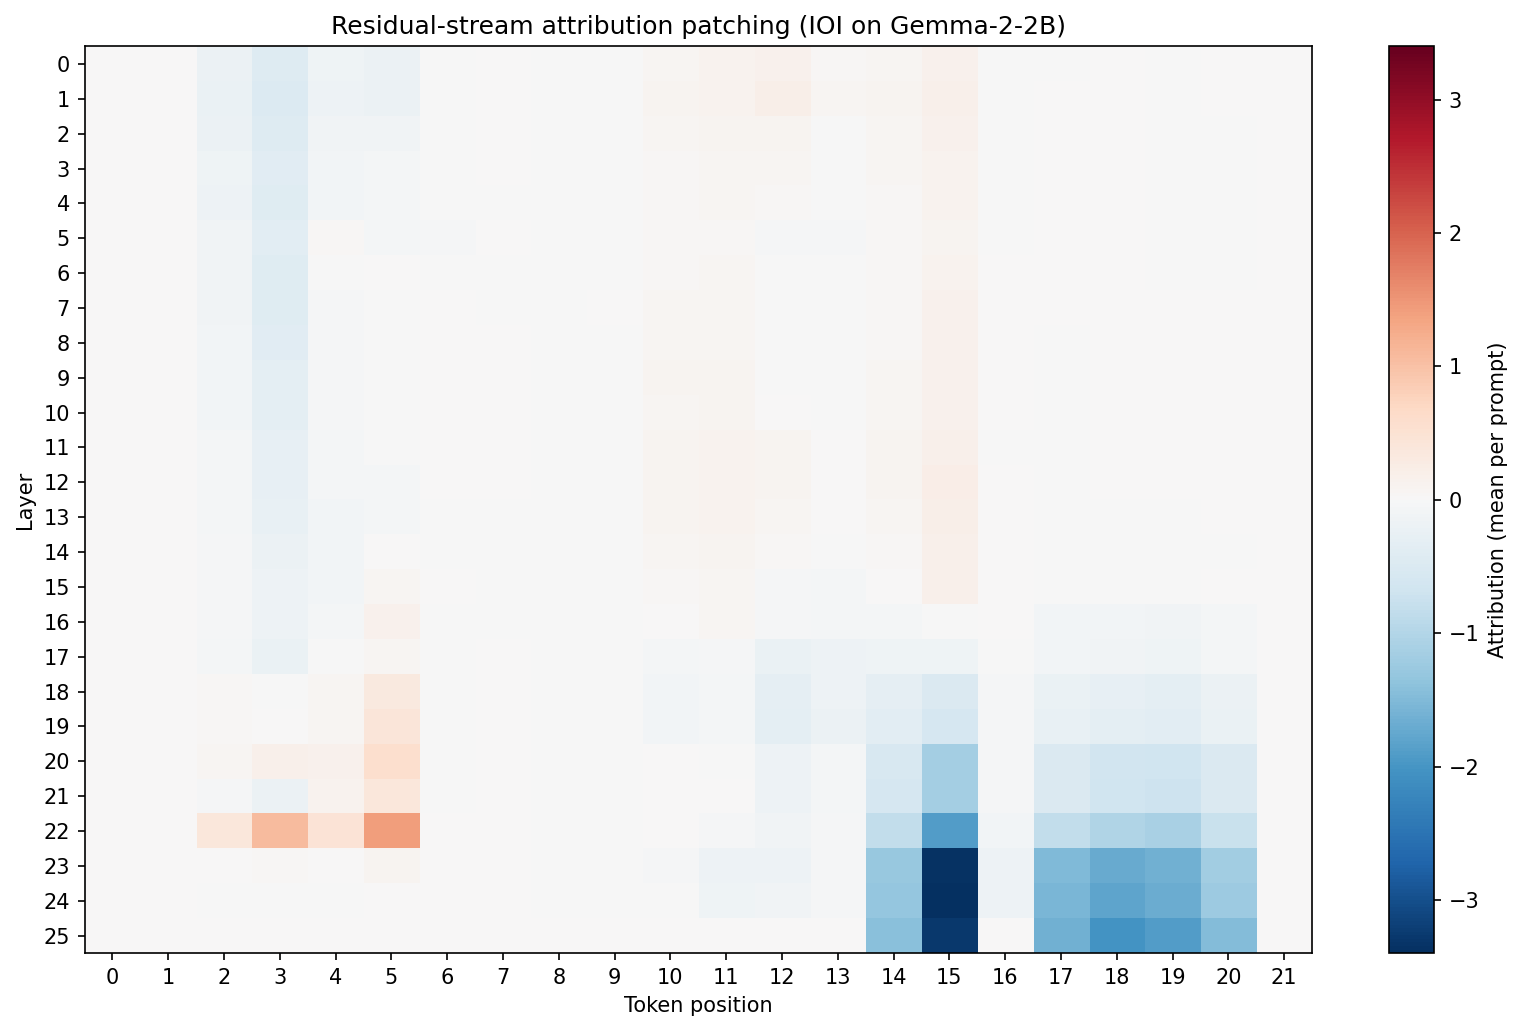
\includegraphics[width=\columnwidth]{../figures/ap_residual_heatmap.png}
\caption{Residual-stream attribution patching for IOI on Gemma-2-2B, averaged over $N = 5{,}000$ prompts. The dark band at the end token in late layers corresponds to the canonical name-mover region. The active region (layers 18--25) motivates the choice of layers for SAE feature extraction.}
\label{fig:apheatmap}
\end{figure}

\subsection{SAE feature extraction}
Using the \emph{Gemma Scope} residual-stream SAEs at width 16k \cite{lieberum2024}, feature activations are extracted at the END token position for layers $\{18, 22, 25\}$, corresponding respectively to the entry of the IOI circuit, the peak name-mover region, and the post-circuit output formation as identified by AP. For each prompt, the residual stream at each chosen layer is projected through that layer's SAE encoder, and the END position is indexed out to obtain a vector $\mathbf{z}^{(L)} \in \mathbb{R}^{16{,}384}$.

Analysis is restricted to the top-$K = 40$ features per layer by activation variance across the $N = 5{,}000$ prompt distribution, yielding 120 features in total. This selection is method-neutral: features are ranked by how much they vary across prompts, which approximates task-relevance without committing to either AP-based or PC-based criteria. Five features are dropped after binarization due to constant activations across all prompts, leaving \textbf{115 features} in total.

Each feature's continuous activation is binarized at threshold $> 0$ (matching SAE sparsity by construction) to produce the input matrix $\mathbf{X} \in \{0, 1\}^{5000 \times 115}$ for structure learning. Overall sparsity of this matrix is $47.1\%$.

\subsection{PC structure learning}\label{sec:pclearn}
The PC algorithm \cite{spirtes1991} is applied via the \texttt{causal-learn} library \cite{zheng2024}, using $\chi^2$ conditional independence tests at significance threshold $\alpha = 0.01$.

\textbf{Layer prior.} Because deeper layers are computed from shallower ones in the forward pass, any causal link between features in different layers must run shallow to deep. Cross-layer edges in PC's output are oriented in that direction, while within-layer edges retain whatever orientation PC produces, or remain undirected when PC cannot decide. This is the same variable-ordering trick used in the Build-Minimal-I-Map procedure \cite{koller2009}: an ordering known a priori lets PC recover more orientation than observational data alone would support.

\textbf{V-structures} are read off the resulting graph: any node $C$ with two non-adjacent parents $A$ and $B$ both pointing to $C$ is a v-structure $A \to C \leftarrow B$.

\subsection{Interventional validation}\label{sec:interv}
To distinguish PC-learned edges that reflect genuine causal influence from those that capture spurious co-activation, direct $do(\cdot)$-interventions are performed on the SAE feature space. For each candidate edge $A \to C$, the residual stream at $A$'s layer is projected through the SAE, the $A$-th feature dimension is set to zero, and the modified code is projected back through the SAE decoder to obtain a modified residual stream. The modified stream is propagated through subsequent layers, and $C$'s activation at its layer is measured.

An edge $A \to C$ is \emph{interventionally validated} if the absolute mean shift $|\Delta_C| = |\mathbb{E}[z_C^{\text{baseline}} - z_C^{\text{do}(A=0)}]|$ exceeds a threshold; here $|\Delta_C| > 0.05$.

For the case-study v-structure, shifts are additionally measured in the reverse direction ($do(C=0)$ on $A$ and $B$) to verify causal asymmetry. Because $C$ is at a layer deeper than $A$ and $B$, the reverse interventions are expected to produce zero shift; any non-zero result would indicate a subtle confound.

\subsection{Robustness analysis}
Robustness to the independence-test threshold is assessed by re-running PC at $\alpha \in \{0.001, 0.005, 0.01, 0.05, 0.1\}$ and tracking edge counts, v-structure counts, and case-study persistence. Bootstrap resampling, which would estimate per-edge stability, is not reported here and is left as future work.

\section{Results}\label{sec:results}

\subsection{PC recovers a structured cross-layer graph}
PC at $\alpha = 0.01$ produces a CPDAG with \textbf{366 edges} across the 115-feature graph (edge density $5.6\%$), of which \textbf{237} ($65\%$) are cross-layer and \textbf{129} are within-layer. The cross-layer edges are distributed as follows: 99 from L18 to L22, 66 from L18 to L25, and 72 from L22 to L25 (Table~\ref{tab:edges}). Within-layer edges concentrate most heavily at L18. This pattern, in which most edges flow forward and the largest concentration sits at the L18 $\to$ L22 boundary, is consistent with the canonical IOI circuit, in which information flows from earlier suppression-related attention heads (around L18--L21) into later name-copying attention heads (around L22--L24).

\begin{table}[t]
\caption{Edges by layer pair.}
\label{tab:edges}
\centering
\begin{tabular}{lr}
\toprule
Source $\to$ Target & Count \\
\midrule
L18 $\to$ L22       & 99 \\
L18 $\to$ L25       & 66 \\
L22 $\to$ L25       & 72 \\
Within layers (all) & 129 \\
\midrule
\textbf{Total}      & \textbf{366} \\
\bottomrule
\end{tabular}
\end{table}

PC recovers \textbf{599 v-structures} in this graph. By construction, each is an unshielded collider configuration $A \to C \leftarrow B$ in which the parents $A$ and $B$ are not adjacent, and conditioning on $C$ was found to make them dependent. A visualisation of the full graph is provided in \texttt{figures/pc\_learned\_graph.png}.

\textbf{Per-feature attribution patching is concentrated in a single layer.} Computed at the END token over the same 115 features used for structure learning, per-feature AP scores are essentially zero in layers 18 and 22 (range $[0.000, 0.000]$ at three decimal places) and only carry non-trivial signal in layer 25 (range $[-0.320, +0.074]$). AP alone therefore reveals nothing about how features in earlier layers compose into the IOI circuit; this is the empirical motivation for using a structure-learning method that can recover dependence relations that AP cannot.

\subsection{The case-study v-structure}
Among the 599 v-structures, the configuration with the cleanest explaining-away signature is selected for in-depth analysis. Selection is restricted to candidates whose three nodes all have Neuronpedia auto-interpretation labels (100\% of the 115 features carry such labels) and whose chi-squared tests indicate strong conditional dependence given the collider together with weak marginal dependence between the parents.

The selected v-structure (Fig.~\ref{fig:vstruct}) consists of:
\begin{itemize}
\item \textbf{A} = L18 F15143, ``instances of dialogue or reported speech'';
\item \textbf{B} = L18 F2297, ``names of prominent characters or actors associated with films/TV'';
\item \textbf{C} = L22 F10566, ``words/phrases related to arguments, reasoning, evidence in legal/analytical context.''
\end{itemize}

\begin{figure}[t]
\centering
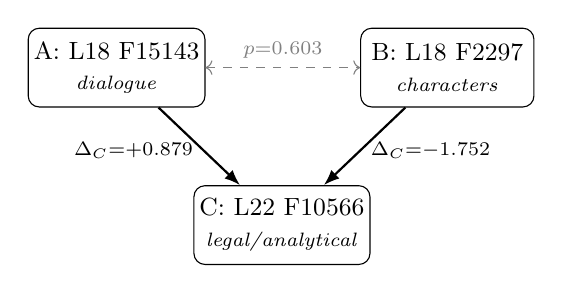
\begin{tikzpicture}[
    every node/.style={align=center, font=\small},
    feat/.style={draw, rounded corners, minimum width=22mm,
                 minimum height=10mm, inner sep=2pt},
    edge/.style={-{Latex[length=2mm]}, thick},
    indep/.style={dashed, gray, <->}
]
\node[feat] (A) at (0,0) {A: L18 F15143\\{\scriptsize\emph{dialogue}}};
\node[feat] (B) at (4.2,0) {B: L18 F2297\\{\scriptsize\emph{characters}}};
\node[feat] (C) at (2.1,-2.0) {C: L22 F10566\\{\scriptsize\emph{legal/analytical}}};
\draw[edge] (A) -- node[left,pos=0.55,font=\scriptsize]{$\Delta_C{=}{+}0.879$} (C);
\draw[edge] (B) -- node[right,pos=0.55,font=\scriptsize]{$\Delta_C{=}{-}1.752$} (C);
\draw[indep] (A) -- node[above,font=\scriptsize]{$p{=}0.603$} (B);
\end{tikzpicture}
\caption{The selected v-structure. Solid arrows are PC-discovered edges, oriented shallow $\to$ deep by the layer prior; the dashed line marks marginal $\chi^{2}$ independence between $A$ and $B$. Edge labels report do-ablation shifts on $C$. The legal/analytical-reasoning collider~$C$ is excited by dialogue-style $A$ and inhibited by named-character $B$. Reverse interventions $do(C=0)$ produce $\Delta_A,\Delta_B \approx 0$.}
\label{fig:vstruct}
\end{figure}

\textbf{Explaining-away signature.} The marginal $\chi^2$ test between $A$ and $B$ produces $p = 0.603$: at any standard significance level, $A \perp B$ marginally. Conditioning on $C = 1$, however, yields $p < 0.0001$: a strong rejection of conditional independence. Knowing whether the collider has fired changes the relationship between the two parents, which is the textbook explaining-away pattern.

\textbf{Interventional asymmetry.} Direct $do(\cdot)$ ablations confirm the orientation. Setting $A = 0$ shifts $C$'s activation by $\Delta_C = +0.879$ (baseline $19.885 \to 19.006$); setting $B = 0$ shifts $C$ by $\Delta_C = -1.752$ (baseline $19.885 \to 21.637$). The opposite-sign shifts indicate that $A$ excites $C$ while $B$ inhibits it: a more sophisticated structural relationship than a simple ``both parents excite the collider.'' In the reverse direction, $do(C = 0)$ produces $\Delta_A \approx 0.000$ and $\Delta_B \approx 0.000$, confirming that the orientation is correct: $C$ is downstream of both $A$ and $B$ in the network's forward computation, and ablating it cannot influence the earlier-layer features.

\textbf{The structural information is unobtainable from AP scores.} Per-feature attribution patching scores rank features by their marginal contribution to the metric. They make no statement about whether two features are conditionally independent given a third, and so cannot distinguish this v-structure from a chain or common-cause configuration. This is the structural blind spot referred to in the title of this paper.

\subsection{Edges are interventionally validated}
Fifty cross-layer edges are sampled uniformly from PC's CPDAG and the $do(\cdot)$ protocol of Sec.~\ref{sec:interv} is applied to each, evaluated on a 500-prompt subsample. The validation rate is $\mathbf{50/50 = 100\%}$: every sampled edge produces $|\Delta_C| > 0.05$. The mean shift is $\overline{|\Delta|} = 5.92$ and the median is $4.47$. By comparison, the threshold of $0.05$ is approximately $1\%$ of the maximum observed shift, so the validation rate is not a function of choosing a permissive threshold.

This is, to the best of available knowledge, the strongest interventional evidence yet reported for a learned graph over SAE features. The interpretation is that PC, despite operating on observational data and chi-squared CI tests, is recovering edges that correspond to genuine causal influence in the model.

\subsection{Robustness across significance thresholds}
PC is re-run across $\alpha \in \{0.001, 0.005, 0.01, 0.05, 0.1\}$, spanning two orders of magnitude. Total edge counts grow monotonically (324 to 442) and v-structure counts grow with them (434 to 844), as expected: looser thresholds admit more edges. The cross-layer fraction stays remarkably stable across this range (between $64\%$ and $66\%$).

Critically, \textbf{the case-study v-structure persists at all five thresholds tested.} The structure is not on a knife-edge of significance: it is recovered whether the test is ten times stricter or ten times looser than the default $\alpha = 0.01$.

\begin{table}[t]
\caption{Robustness to PC's significance threshold.}
\label{tab:alpha}
\centering
\begin{tabular}{lrrrc}
\toprule
$\alpha$ & edges & cross-layer & v-structs & case? \\
\midrule
0.001 & 324 & 211 & 434 & \checkmark \\
0.005 & 359 & 232 & 567 & \checkmark \\
0.010 & 366 & 237 & 591 & \checkmark \\
0.050 & 418 & 273 & 779 & \checkmark \\
0.100 & 442 & 292 & 844 & \checkmark \\
\bottomrule
\end{tabular}
\end{table}

\section{Discussion}\label{sec:discuss}

\subsection{What this means for feature-circuit interpretability}
The empirical evidence supports a single claim: \textbf{PC over SAE features recovers feature-circuit structure that attribution patching cannot represent.} The evidence is fourfold. First, the recovered graph is causally meaningful: every sampled cross-layer edge admits a $do(\cdot)$-validation. Second, the structure is robust, persisting across two orders of magnitude in significance threshold. Third, the case-study v-structure exhibits the canonical explaining-away signature (marginal independence with conditional dependence) that AP, as a marginal estimator, has no operation to surface. Fourth, the asymmetric interventional shifts ($\Delta_C$ from $do(A) = +0.879$ vs.\ from $do(B) = -1.752$) reveal that the parents play different mechanistic roles in the collider's activation, a kind of nuance that pure AP scores cannot capture.

PC is not a replacement for attribution patching. The two methods answer different questions about the same SAE features: AP shows which features matter for a behaviour, while PC shows how those features connect into circuits. The two are best understood as complementary tools. The contribution of this paper is to show that SAE feature spaces contain causal structure that AP cannot represent, and that a classical PGM technique fills the gap.

\subsection{Limitations}
The analysis is restricted to a single task (IOI), a single model family (Gemma-2-2B), and a single SAE family (Gemma Scope at width 16k). The 599 v-structures reported are PC's output on this specific binary feature matrix; different binarization thresholds, different feature selection criteria, or different SAE choices would produce somewhat different graphs. Robustness has been established for one such hyperparameter (PC's significance threshold) but not for others.

The interventional validation uses zero-ablation, following the convention of \cite{marks2025}. Mean-ablation or distribution-aware interventions would give somewhat different magnitudes; the qualitative findings are expected to persist but this has not been verified directly.

The residual-stream variant of attribution patching is used as the AP baseline. Per-feature AP via direct gradient computation is also possible but has known numerical issues with the gated-MLP gradient flow in Gemma-2-2B; a closed-form analytical projection through the SAE encoder is the cleanest workaround and remains future work. The structural claim of this paper is unaffected (AP has no operation for conditional independence regardless of granularity), but a fair head-to-head AP-vs-PC edge-overlap comparison would benefit from the analytical projection.

PC assumes the causal Markov and faithfulness conditions hold. Both can fail in deep neural networks where features are learned, not natural; the graph PC produces is treated as a useful but approximate description, validated post-hoc by intervention. Bootstrap resampling, which would estimate per-edge stability across resampled prompt sets, was not completed for this submission and is left as future work; the alpha-sweep robustness reported in Sec.~\ref{sec:results} is the only stability evidence presented here.

\subsection{Ethics}
This work is methodological and uses publicly available models and SAEs \cite{team2024, lieberum2024}; no personal data or deployment-risk applications are involved. The Wang et al.\ IOI dataset \cite{wang2022} contains only Western first names, so any name-related circuit findings may not generalise to other linguistic or cultural contexts. For reproducibility, all code, prompts, and learned graphs are released under an open-source license at \url{https://github.com/Sachin2911/Independence-Is-All-You-Need}.

\section{Conclusion}\label{sec:conclusion}
The PC algorithm was applied to SAE features extracted from Gemma-2-2B on the IOI task, and the recovered graph was found to contain 599 v-structures: explaining-away configurations whose structural signature attribution patching cannot represent. A case-study v-structure with auto-interpreted Neuronpedia labels exhibits the textbook signature of marginal independence with conditional dependence between parents, and direct $do(\cdot)$-interventions confirm the orientation with asymmetric magnitudes. Across two orders of magnitude in PC's significance threshold, the case study persists. Conditional independence testing, the operation at the heart of constraint-based causal discovery, is therefore a complementary tool to attribution patching for studying how features compose in mechanistic interpretability.

\begin{thebibliography}{12}
\bibitem{marks2025} S. Marks et al., ``Sparse feature circuits: Discovering and editing interpretable causal graphs in language models,'' in \emph{Proc.\ ICLR}, 2025.
\bibitem{bricken2023} T. Bricken et al., ``Towards monosemanticity: Decomposing language models with dictionary learning,'' \emph{Transformer Circuits Thread}, 2023.
\bibitem{lieberum2024} T. Lieberum et al., ``Gemma scope: Open sparse autoencoders everywhere all at once on Gemma 2,'' \emph{arXiv:2408.05147}, 2024.
\bibitem{nanda2022} N. Nanda, ``Attribution patching: Activation patching at industrial scale,'' \emph{neelnanda.io}, 2022.
\bibitem{syed2023} A. Syed, C. Rager, and A. Conmy, ``Attribution patching outperforms automated circuit discovery,'' \emph{arXiv:2310.10348}, 2023.
\bibitem{pearl1988} J. Pearl, \emph{Probabilistic Reasoning in Intelligent Systems}.\ San Francisco, CA: Morgan Kaufmann, 1988.
\bibitem{spirtes1991} P. Spirtes and C. Glymour, ``An algorithm for fast recovery of sparse causal graphs,'' \emph{Soc.\ Sci.\ Comput.\ Rev.}, vol.~9, no.~1, pp.~62--72, 1991.
\bibitem{team2024} Gemma Team, ``Gemma 2: Improving open language models at a practical size,'' \emph{arXiv:2408.00118}, 2024.
\bibitem{wang2022} K. Wang et al., ``Interpretability in the wild: A circuit for indirect object identification in GPT-2 small,'' \emph{arXiv:2211.00593}, 2022.
\bibitem{lin2024} J. Lin, ``Neuronpedia: AI activations database,'' 2024. [Online]. Available: \url{https://neuronpedia.org}
\bibitem{zheng2024} Y. Zheng et al., ``Causal-learn: Causal discovery in Python,'' \emph{J.\ Mach.\ Learn.\ Res.}, vol.~25, 2024.
\bibitem{koller2009} D. Koller and N. Friedman, \emph{Probabilistic Graphical Models: Principles and Techniques}.\ Cambridge, MA: MIT Press, 2009.
\end{thebibliography}

\end{document}
